%Kelompok Memory Allocation (2)
%Arjun Yuda Firwanda
%Dezha Aidil Martha
%Dwi Septiani Tsaniyah
%Muh.Rifky Prananda
%Yusuf Al-Qordhawi

Putty

\section {Membahas Tentang "Putty"}

\subsection {A. Memahami Putty}

Putty adalah program open source yang dapat digunakan untuk melewati protokol jaringan SSH (Secure Shel), Telnet dan Rlogin. Protokol ini dapat digunakan untuk remote pada komputer melalui jaringan, baik LAN (Local Area Network) atau internet. Program ini digunakan oleh pengguna komputer saat ini, sekarang untuk menghubungkan, mensimulasikan, dan masalah yang terkait dengan jaringan. Program ini tentu saja juga sebagai sebuah terowongan (enkapsulasi atau pembungkusan protokol) di dalam jaringan.
Protokol dapat digunakan untuk mengetahui jaringan atau menjalankan sesi jarak jauh di komputer.

\begin{enumerate}

	\item SSH (Secure Shell)
	Merupakan protokol jaringan yang memungkinkan pertukaran data melalui saluran aman antara dua perangkat jaringan.

	\item Rlogin
	Sistem yang memungkinkan kita dapat masuk dari satu sistem ke sistem lain tanpa kata sandi tambahan.

	\item Telnet
	Adalah jaringan telekomunikasi yang digunakan di Internet atau Local Area Network (LAN) untuk menyediakan fasilitas komunikasi berbasis teks yang menggunakan koneksi terminal virtual.

\end{enumerate}


\subsection {Mengetahui Lebih dalam Putty}

PuTTY adalah alat komunikasi antara pengguna dengan server yang dipergunakan oleh pemilik server untuk berkomunikasi dengan server mereka atau server lain dengan menggunakan perintah teks yang berguna untuk menjalankan perintah tertentu. Artinya dengan perintah teks si pemilik server dapat berkomunikasi dengan servernya tanpa ada kendala dalam konfigurasi dengan system.

"PuTTY adalah klien SSH dan telnet, yang dikembangkan awalnya oleh Simon Tatham untuk platform Windows PuTTY adalah perangkat lunak open source yang tersedia dengan kode sumber dan dikembangkan dan didukung oleh sekelompok relawan.
- www.putty.org "

Tujuan utama PuTTY adalah menjadi aplikasi multi-platform (aplikasi yang bisa dijalankan diOperating System apa saja) yang mampu menjalankan sistem operasi. Dan Ia juga dapat disebut terminal xterm (emulator).

Jendela utama PuTTY memiliki sesi yang berjalan di komputer jarak jauh dan dapat mengirim perintah langsung ke komputer jarak jauh, melalui konfigurasi system. Artinya dengan alat ini dapat dijalankan dengan jarak jauh melalui konfigurasi dengan system.

PuTTY memberikan beberapa keunggulan yang berbeda, terutama dari jarak jauh. Lebih mudah untuk mengalami. Pada saat yang sama memfasilitasi pengembang untuk mengembangkan aplikasi yang sesuai dengan kebutuhan sistem saat ini. 

\begin{figure}[ht]
\centerline{
\includegraphics[width=1\textwidth]{figures/puttyexe.jpg}}
\caption{gambar putty.}
\label{putty}
\end{figure}

\subsection {Tips menggunakan Aplikasi Putty}
Di sini adalah Tips menggunakan Aplikasi Putty dengan mudah
1. Unduh Aplikasi Putty di www.putty.org
2. Jika sudah di unduh, Letakkan Aplikasi Putty.exe ke dalam folder C:\Windows
3. Lalu buat shortcut di desktop dengan klik kanan di desktop lalu add shortcut dan browse aplikasi Putty yang sudah anda unduh
4. Setelah shortcut dibuat, Jalankan Putty.exe dengan klik kanan dan run as administrator.
5. Jika sudah, Lanjut ke pengaturan putty dan atur seperti ini
Mengatur Koneksi Putty :
* Hostname 			: Ip Address
* Port 				: 22
* Connection type 	: SSH
6. Lalu klik Open untuk menjalankan sesi SSH
7. Akan muncul notifikasi bahwa anda untuk pertama kalinya login ke server menggunakan Putty, Pilih Yes untuk melanjutkan.
8. Setelah masuk ke dalam laman awal koneksi SSH Terminal. akan di beri prompt untuk memasukkan username SSH.
9. Lalu masukkan password SSH dan akan nampak ketikan password di terminal tidak terketik. Perlu diingatkan aplikasi terminal tetap menerima ketikan anda walaupun tidak terlihat. Jika masih ragu untuk memasukan password, gunakan Ctrl+C pada bagian kata yang di cap untuk memasukkan password lalu Ctrl+V.
10. Jika sudah memasukkan username dan password SSH, maka anda sudah berhasil login ke server melalui SSH.
 
\subsection {Pengertian Rlogin (Remote Login)}

Rlogin atau Remote Login merupakan salah satu dari berbagai macam layanan internet yang memungkinkan pengguna internet untuk mengakases (masuk)  sebuah host dalam lingkup jaringan internet, seorang user dapat mengoperasikan sebuah host dari jarak jauh tanpa harus kontak secara fisik dengan host. Di sana user dapat melakukan maintenance atau pemeliharaan, menjalankan sebuah program, bahkan menginstall program baru di host.

Protokol yang sering di gunakan untuk keperluan Rlogin adalah Telnet (Telecommunication network) yang berjalan pada port 23. Namun Rlogin lewat Telnet memiliki resiko keamanan karena data yang dikirimkan dalam bentuk plain text (tidak dienkripsi). Untuk user / pengguna (cracker bisa di masukkan kategori pengguna) yang dapat menangkap paket pada suatu jaringan (Sniffing), bisa mengambil berbagai macam informasi mengenai host dan remote host.


\begin{figure}[ht]
\centerline{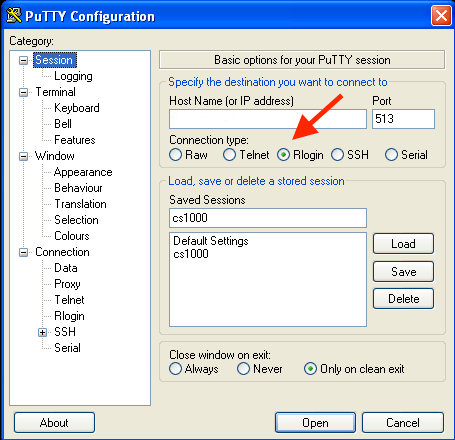
\includegraphics[width=1\textwidth]{figures/rlogin.png}}
\caption{gambar rlogin.}
\label{rlogin}
\end{figure}


\subsection {Pengertian SSH(Secure Shell)}

Menurut pendapat \cite{Jusuf.Heni2015Penggunaan Secure Shell} SSH adalah suatu kriptografi yang digunakan untuk mengkomunikasikan data yang ada pada perangkat jaringannya untuk membuatnya lebih aman lagi. Dalam konsep menggunkan SSH ini harus di dukung oleh suatu server atau di dalam computer. Pada akun SSH ini dirancang untuk digunakan sebagai pola piker Telnet dan shell pada jarak jauh yang tidak aman, yang mengirimkan suatu informasi terutama pada kata sandinya dalam bentuk yang sederhanan dan mudah untuk disadap. Enkripsi disediakan oleh SSH untuk memberikan suatu kerahasiaan dan integritas data melalui jaringan tidak aman seperti internet.

SSH yaitu merupakan protokol jaringan yang menggunakan kriptografi atau yang biasa dikenal sebagai secure shell untuk komunikasi data yang aman. Dalam konsep menggunakan SSH ini harus didukung oleh server atau perangkat komputer yang bertukar data. Buka server SSH Server dari server samping dan SSH client untuk komputer penerima atau klien.
Aplikasi yang terkenal di protokol ini yaitu untuk akses ke akun shell di sistem operasi sama seperti unix, SSH dirancang sebagai telnet yang tidak aman dan pola pikir shell jarak jauh, yang mengirimkan informasi terutama kata sandi dalam bentuk teks sederhana yang mudah diketuk. Protokol ini dibedakan menjadi 2 versi utama yang dikenal sebagai SSH 1 dan SSH 2. Enkripsi yang digunakan oleh SSH bertujuan untuk memberikan rahasia dan integritas data melalui jaringan yang tidak aman seperti internet. 

\begin{figure}[ht]
\centerline{\includegraphics[width=1\textwidth]{figures/ssh.gif}}
\caption{gambar ssh.}
\label{ssh}
\end{figure}


SSH bermanfaat untuk meningkatkan data di komputer melalui internet, karena untuk dengan terhubung ke internet kita menggunakan SSH, SSH akan menyediakan semua data yang bisa dibaca, cukup dengan masuk ke server lain.
Selain untuk enkripsi data, SSH juga memiliki kemampuan untuk melakukan Port Forwarding yang akan kita gunakan sebagai berikut:

1.Menghubungkan aplikasi TCP (misalnya: server web, server email, server FTP) dengan lebih aman (aman)
2.Terhubung dengan firewall atau proxy lokal.

Manfaat kedua diatas itulah yang sering dicari oleh para pengguna Internet dan memanfaatkannya untuk kepentingan akses internet. menggunakan Akun SSH Kita bisa mengelola VPS untuk menjadi hosting ataupun fungsionalitas yang lain.

Menggunakan Akun SSH untuk menggali koneksi internet Anda tidak menjamin peningkatan kecepatan internet Anda. Namun dengan menggunakan Akun SSH, IP otomatis yang Anda gunakan akan statis dan Anda dapat menggunakannya secara pribadi dengan catatan bahwa Anda adalah satu-satunya pengguna di Akun SSH.
Protokol SSH (Secure Shell) memiliki banyak fungsi, selain fungsi tunneling yang sering kita gunakan, kita juga dapat menggunakan SSH (Secure Shell) untuk SFTP, SOCKS4 / 5 proxy atau kita juga dapat menggunakan untuk mengelola VPS (Virtual Private Server) atau hosting kami terutama VPS dengan OS Linux seperti CentOS. Untuk menggunakan tunneling menggunakan SSH (Secure Shell) , kita dapat menggunakan klien SSH (Secure Shell) seperti Bitvise Tunnelier atau Putty untuk sistem operasi Windows.
Untuk mendapatkan akun ini dan menggunakan SSH (Secure Shell), kita bisa mendapatkan akun SSH (Secure Shell) secara gratis di cjb.net atau jika kami memiliki penyedia VPS (Virtual Private Server) biasanya juga menyediakan SSH untuk pengaturan VPS kami.

\subsection {Kegunaan SSH atau Secure Shell}
SSH dirancang untuk membahas protokol telnet dan FTP. SSH adalah produk yang digunakan untuk melakukan banyak hal, paling tepat antara tunnel antar host. Dua hal penting SSH adalah login console (misalnya telnet) dan secure filetransfer (selain FTP), tetapi dengan SSH Anda juga dapat mengakses HTTP, FTP, POP3, dan hal lain melalui SSH tunel.

\subsection {Cara kerja SSH atau Secure Shell}

Kunci publik / pribadi yang masing-masing menjadi identitas SSH untuk keduanya.
Langkah-langkah yang terhubung adalah sebagai berikut:

\begin{enumerate}

	\item Langkah 1 
	Klien mengikat nomor port lokal besar dan menghubungkan ke port 22 di server.

	\item Langkah 2
	Klien dan server setuju untuk menggunakan sesi SSH tertentu. Ini penting karena SSH v.1 dan v.2 tidak kompatibel.

	\item Langkah 3
	Klien akan menjadi server dan kata kunci.

	\ietm Langkah 4
	Klien dan server ditugaskan ke algoritma yang akan digunakan (misalnya TripleDES atau IDEA).

	\item Langkah 5
	Klien yang terdiri dari klien dan enkripsi menggunakan server kunci pribadi mereka sendiri.

	\item Langkah 6
	Server mendekripsi sesi yang diperoleh dari klien, mengenkripsi ulang dengan kunci publik klien, dan mengirimnya kembali ke klien untuk verifikasi.

	\item Langkah 7
	Pengguna mengotentikasi dirinya ke server dalam aliran data terenkripsi di kunci sesi. Sampai di sini, koneksi telah dibuat, dan klien dapat bekerja secara interaktif di server atau mentransfer file ke atau dari server. Langkah ketujuh dapat diimplementasikan dengan berbagai cara (nama pengguna, kerberos, RSA dan lainnya).

\end{enumerate}
	
\subsection {SSH,Telnet,dan Rlogin}

SSH, Telnet, dan Rlogin

SSH, Telnet, dan Rlogin sebenarnya memiliki fungsi yang sama: login (login) ke komputer multi-pengguna (server) dari komputer lain (klien) melalui jaringan. Sistem operasi multi-pengguna, seperti Unix dan VMS, biasanya menyediakan antarmuka pengguna langganan, yang tampak seperti 'command prompt' atau 'MS-DOS prompt' di Windows. Sistem menampilkan prompt dan kami mengetikkan perintah yang akan dijalankan oleh sistem.
Dengan cara komunikasi client-server seperti ini, kita tidak perlu mengakses (baca: sentuh) langsung sistem komputer server. Perintah dan tanggapan dapat dikirim melalui jaringan, sehingga kami dari jarak jauh dapat memberikan perintah ke komputer lain. Bukan hanya satu komputer, bahkan lebih dari satu komputer bisa kita perintah.
SSH, Telnet, dan Rlogin adalah protokol jaringan yang memungkinkan semuanya. Kami hanya perlu menjalankan aplikasi klien, yang akan membuat koneksi ke komputer lain sebagai server. Ini adalah jaringan komputer yang mengirim perintah dari klien ke server, dan mengembalikan respons.

Protokol ini dapat digunakan untuk jenis sesi interaktif berbasis keyboard lainnya. Banyak papan buletin, sistem pembicara, dan MUD (ruang bawah tanah multi-pengguna) adalah dukungan (dapat diakses) dengan Telnet. Tetapi hanya sedikit dukungan SSH.

Kita dapat menggunakan SSH, Telnet, atau Rlogin jika:

    memiliki akun pada sistem Unix atau VMS yang akan kami akses dari tempat lain
    ISP kami memberikan akun login di server web. Ini umumnya dikenal sebagai akun shell. Shell adalah program yang berjalan di server dan menerjemahkan perintah kami.
    kami ingin menggunakan papan buletin, pembicara, atau sistem MUD yang dapat diakses menggunakan Telnet.

Namun, kami tidak dapat menggunakan SSH, Telnet atau Rlogin jika:

    hanya menggunakan Windows. Komputer Windows memiliki cara komunikasi sendiri antara Windows.

	Berikut adalah perbedaan antara SSH, Telnet, dan Rlogin :

1. SSH (secure shell 'dormitory) yang dibuat adalah protokol tingkat tinggi. SSH menggunakan kriptografi yang kuat untuk melindungi koneksi dari penyadapan, pembajakan, atau serangan lainnya. Telnet dan Rlogin adalah protokol pertama yang hadir dan hanya menyediakan tingkat minimal.
2. SSH dan Rlogin memungkinkan kami masuk ke server tanpa mengetikkan kata sandi. (Metode Rlogin sangat aman / tidak aman, memungkinkan penyerang untuk mengakses data di server sementara metode SSH lebih aman sehingga penyerang / penyerang harus mengakses komputer klien secara langsung untuk mengakses akun kami.)
3. Dengan SSH, kita dapat terhubung ke server dan secara langsung secara otomatis, perintah server akan menjalankan perintah dan memutuskan secara otomatis juga. Dengan model ini, kita bisa melakukan pengumpulan otomatis.


\subsection {Fungsi dan Kegunaan}

Fungsi SSH bisa dipakai untuk menggantikan kinerja dari Telnet, RLogin, FTP, dan RSH. Sehingga salah satu fungsi utama dari SSH adalah untuk menjamin keamanan ketika melakukan transmisi / transfer data pada suatu jaringan. SSH banyak dimanfaatkan pada Tipe Jaringan dengan jarak jangkauan yang jauh untuk mengkontrol web dan jenis jaringan lainnya, seperti WAN (Wide Area Network). Fungsi dari SSH ini sendiri sebenarnya dibuat untuk menggantikan fungsi dari protokol jaringan sebelumnya yang dianggap sangat rentan akan terjadinya crash (pencurian data) melalui malware-malwere yang berbahaya.

Karena perkembangan jaringan komputer yang terus membaik, perintah telnet pun dapat dilakukan tanpa harus mengetahui dimana letak telnet berada. Protocol Telnet memiliki beberapa fungsi utama yang banyak digunakan. Fungsi-fungsi tersebut diantaranya ialah :
* Mengakses server atau host secara remote
* Mengubah komputer user menjadi komputer terminal
* Menjalankan komputer menggunakan Telnet jarak jauh


\subsection {Perbedaan Telnet Dengan SSH atau Secure Shell}

Telnet (Telecommunications Network Protoco) l adalah login jarak jauh atau sistem otomatis ketika pengguna menggunakan jaringan Internet sebagai login jarak jauh yang terjadi pada jaringan Internet karena layanan dari protokol Telnet. Telnet dapat memungkinkan pengguna untuk mengakses komputer lain dari jarak jauh melalui Internet. Telnet digunakan untuk login ke komputer lain di Internet dan dapat mengakses layanan publik, termasuk berbagai database. Pengguna hanya bisa duduk di depan komputer yang terhubung ke jaringan internet. Dengan kata lain dapat dihubungkan ke komputer lain di satu gedung, satu ruangan atau bahkan di komputer di seluruh dunia. Setelah terhubung ke jaringan internet Anda di komputer maka masukan yang diberikan pada keyboard dapat langsung mengontrol ke komputer jarak jauh sebelumnya, dapat diakses ke semua layanan yang telah disediakan oleh mesin jarak jauh dan hasilnya akan ditampilkan di terminal lokal. Dengan menggunakan Telnet, pengguna dapat mengakses berbagai layanan seperti melihat katalog perpustakaan dan banyak layanan lainnya. Telnet menggunakan 2 (dua) program pada klien dan server. Program pada klien digunakan untuk meminta layanan pada server, sedangkan program di server akan menyediakan layanan yang diminta oleh klien.

\subsection { Definisi Sederhana }

Definisi sederhana dari aplikasi aplikasi PuTTY adalah Anda menjalankan PuTTY pada OS Windows, dan dapat digunakan untuk menghubungkan (misalnya) mesin Unix. Aplikasi Jendela Putty. Kemudian, apa yang diketik di jendela yang langsung dikirim ke mesin Unix, dan semua jawaban dari OS Unix akan dikirim kembali ke desktop Anda. Jadi Anda dapat bekerja pada mesin Unix jika Anda berada di konsol, padahal sebenarnya tidak ..
Sebelum versi 0.58, tiga rilis berturut-turut (0,55-0,57) dibuat untuk memperbaiki aplikasi yang paling signifikan dalam versi sebelumnya, beberapa aplikasi bug PuTTY bahkan mengizinkan klien untuk masuk di server tanpa validasi terlebih dahulu. Versi 0,58, dirilis pada bulan April 2005, berisi beberapa fitur baru


Dengan Putty, ini memungkinkan kita untuk menerima data dari server komputer lain. Program ini ditemukan pada Oktober 2000 oleh Simon Tatham. Aplikasi ini dapat digunakan kapan saja, tidak ada jaringan internet atau offline. Dengan kata lain, cara menggunakan Putty sederhana dan "tidak aneh", manfaatnya adalah bahwa kita dapat menerima data dari komputer lain PUTTY adalah aplikasi yang bertindak sebagai pelanggan untuk menerima data, mengirim data, dan menghubungkan komputer dari jarak jauh menggunakan Port SSH dll. Aplikasi PUTTY menyediakan data dan data dari komputer 1 ke komputer lain